\section{Proposed approach}
\label{sec:apprach}

Given a set of existing DSLs  our approach is intended to identify a catalog of reusable language modules from a given set of DSLs (that we refer to as the \textit{input set}). To this end, our approach is threefold (see Figure \ref{fig:breakingdown}). \textbf{First}, we identify commonalities existing in a given set of DSLs. Those commonalities are structured as the form of Venn diagrams containing syntax and semantic overlapping. \textbf{Second}, we break-down the Venn diagrams by separating all the intersections; for each different intersection, we create a language module by considering not only syntax but also semantics. \textbf{Third}, we encapsulate those language modules and we establish the dependencies among them by means of interfaces. The reminder of this section is dedicated to deeply explain our approach. 

\begin{figure}
\centering
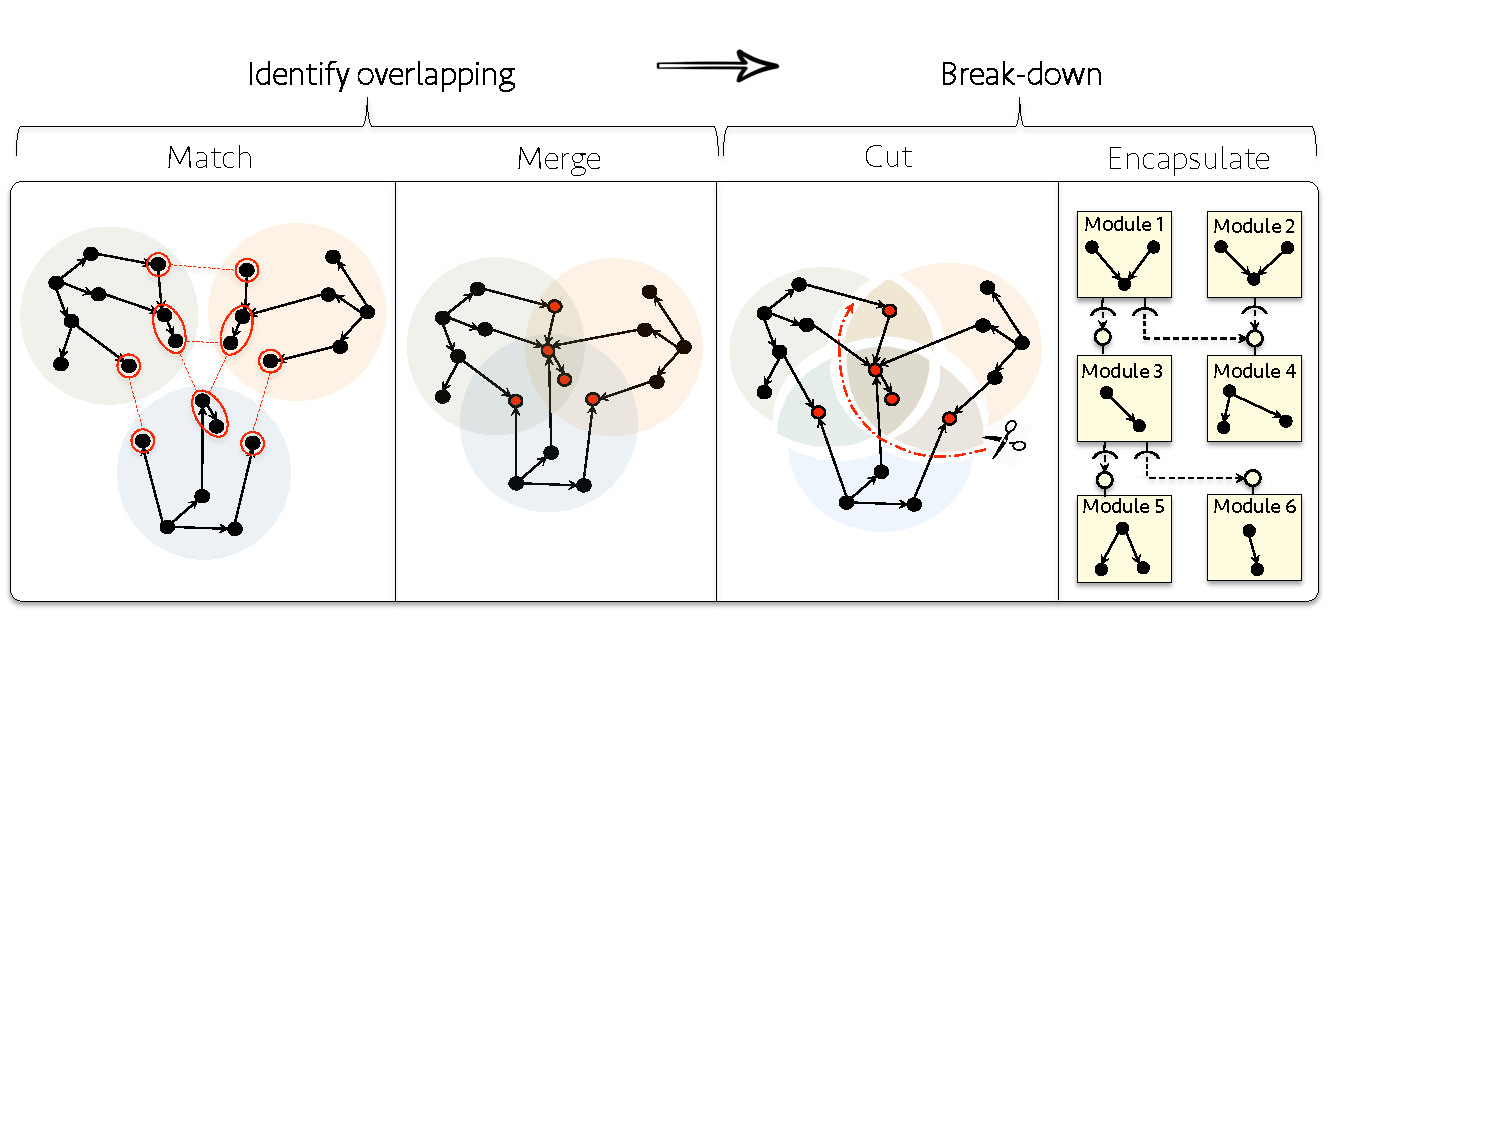
\includegraphics[width=1\linewidth]{images/breakdown.pdf}
\caption{Breaking down the input set by separating overlapping}
\label{fig:breakingdown}
\end{figure}

\subsection{Identifying overlapping}
\label{sec:metrics}
\todo[inline]{Donde esta el algoritmo?? parece que cuentas de nuevo lo de arriba. Toca hablar de como comparas los lenguages y generas el grafo para despues partirlo. Parece naive una cosa que no lo es. Se que lo haces por que eres buen profe, pero aqui hay que sacar pecho de lo super-mega-dificil que es.}
Our algorithm for identifying \textbf{syntactic overlapping} can be described as by the function that receives a set of metamodels (one for each DSL of the input set) and returns a set of tuples containing all the overlapping (i.e., metaclasses that are \textit{equal}) among these metamodels. Note that there can be overlapping among any of the combinations of the input set. Hence, in the result there is a tuple for each of the possible combinations of the input metamodels (i.e., the power set). Similarly, our algorithm for detecting \textbf{semantic overlapping} can be described as a function that receives a set of aspects (one for each DSL of the input set) and returns a set of tuples containing all the overlapping (i.e., domain-specific actions that are \textit{equal}) among these aspects.

%\begin{equation}
%  Venn_{syn} : set(MM) \rightarrow set(<set(MM),set(MC)>)
%\end{equation}

%\begin{equation}
%  Venn_{syn}(mms) = \{<x,y> \mid x \in \mathcal{P}(mms), y = I_{syn}(x)\}
%\end{equation}

%Note that our algorithm relies on a function $I_{syn}$ that computes the intersection existing withing a given set of metamodels. It can be formalized as follows:

%\begin{equation}
%  I_{syn} : set(MM) \rightarrow set(MC)
%\end{equation}
%\vspace{-2mm}
%\begin{equation}
%  I_{syn}(mms) = \bigcap _{i=0}^{|mms|}mms_i
%\end{equation}

%Similarly, our algorithm for detecting \textbf{semantic intersections} can be described as a function that receives a set of aspects (one for each DSL of the input set) and returns a set of tuples containing all the intersections among these aspects. 

%\begin{equation}
%  Venn_{sem} : set(A) \rightarrow set(<set(A),set(DSA)>)
%\end{equation}

%\begin{equation}
%  Venn_{syn}(mms) = \{<x,y> \mid x \in \mathcal{P}(mms), y = I_{sem}(x)\}
%\end{equation}
%\vspace{2mm}

%This time, the algorithm for semantic commonalities relies on a function $I_{sem}$ that computes the intersection existing withing a given set of aspects. It can be formalized as follows:

%\begin{equation}
%  I_{sem} : set(A) \rightarrow set(DSA)
%\end{equation}
%\vspace{-2mm}
%\begin{equation}
%  I_{sem}(dsas) = \bigcap _{i=0}^{|dsas|}dsas_i
%\end{equation}

It is worth noting that a syntactic overlapping is a set of metaclasses that are equal in two or more DSLs. Similarly, a semantic overlapping is a set of domain-specific actions that are equal in two or more DSLs. At this point we need to clearly define the notion of equality between metaclasses and domain-specific actions. That is, we need to establish the criteria under we consider that two metaclasses/domain-specific actions are equal.


\vspace{-3mm}
\subsubsection{Comparison of metaclasses:} The name of a metaclass usually corresponds to a word that evokes the domain concept the metaclass represents. Thus, intuitively one can think that a first approach to compare meta-classes is by comparing their names. Certainly, this approach results quite useful and it is quite probable that, we can find potential reuse.
\todo[inline]{me falta material. donde esta el fdx que representa el operador de igualdad. Explicame cuantos operadores hay, puedo tener mas? Tu solucion cuantos acepta? }
Unfortunately, comparison of metaclasses by using only their names might have some problems. There are cases in which two meta-classes with the same name are not exactly the same since they do not represent the same domain concept or because there are domains that use similar vocabulary. In such cases, an approach that certainly helps is to compare meta-classes not only by their names but also by their attributes and references.

%\begin{equation}
%  \doteq~: MC \times MC \rightarrow bool
%\end{equation}
%\vspace{-1mm}
%\begin{equation}
%\begin{split}
%  MC_{A} \doteq MC_{B} &= true \implies \\
%   & MC_{A}.name = MC_{B}.name
% \end{split}
%\end{equation}

%\begin{equation}
%  \doteqdot~: MC \times MC \rightarrow bool
%\end{equation}
%\vspace{-1mm}
%\begin{equation}
%\begin{split}
%  MC_{A} \doteqdot MC_{B} &= true \implies \\
%   & MC_{A}.name = MC_{B}.name ~ \wedge \\
%   & \forall a_1 \in MC_{A}.attr \mid (\exists a_2 \in MC_{B}.attr \mid a_1 = a_2) ~ \wedge \\
%   & \forall r_1 \in MC_{A}.refs \mid (\exists r_2 \in MC_{B}.refs \mid r_1 = r_2)
%  \end{split}
%\end{equation}

Our comparison operator for metaclasses is quite restrictive. It identifies two metaclasses as a commonality if and only if their specifications are exactly the same. Hence, potential reuse is guaranteed in the sense that we are sure that there are not additional elements to consider. However, we are aware that there are other approaches to compute commonalities within metaclasses. So, at the implementation level our approach is flexible and additional comparison operators such as the surveyed in \cite{Lafi:2011} can be easily incorporated.
\todo[inline]{toca usar el ejemplo con algunos operadores de ejemplo.}
\vspace{-3mm}
\subsubsection{Comparison of domain-specific actions:} Like methods in Java, domain-specific actions have a signature that specifies its contract (i.e., return type, visibility, parameters, name, and so on), and a body where the behavior is actually implemented. In that sense, the comparison of two domain-specific actions can be performed by checking if their signatures are equal. This approach is practical and also reflects potential reuse; one might think that the probability that two domain-specific actions with the same signatures are the same is elevated.

However, during the conduction of this research we realized that there are cases in which signatures comparison is not enough. Two domain-specific actions defined in different DSLs can perform different computations even if they have the same signatures. As a result, we only guarantee potential reuse where we compare also the bodies of the domain-specific actions. Note that such comparison can be arbitrary difficult. Indeed, if we try to compare  the behavior of the actions we will have to deal with the semantic equivalence problem that, indeed, is known as be undecidable \cite{Lucanu:2013}. In this case, we a conservative approach is to compare only the structure (abstract syntax tree) body of the domain-specific action. To this end, we use the API for java code comparison proposed in \cite{Biegel:2010}.

%\begin{equation}
%  \circeq~: DSA \times DSA \rightarrow bool
%\end{equation}
%\vspace{-1mm}
%\begin{equation}
%\begin{split}
%  DSA_{A} & \circeq DSA_{B} = true \implies \\
%   & DSA_{A}.name = DSA_{B}.name ~ \wedge \\
%   & DSA_{A}.returnType = DSA_{B}.returnType ~ \wedge \\
%   & DSA_{A}.visibility = DSA_{B}.visibility ~ \wedge \\
%   & \forall p_1 \in DSA_{A}.params \mid (\exists p_2 \in %DSA_{B}.params \mid p_1 = p_2)
% \end{split}
%\end{equation}

%\begin{equation}
%  \triangleq~: DSA \times DSA \rightarrow bool
%\end{equation}
%\vspace{-1mm}
%\begin{equation}
%\begin{split}
%  DSA_{A} & \circeq DSA_{B} = true \implies \\
%   & DSA_{A}.name = DSA_{B}.name ~ \wedge \\
%   & DSA_{A}.returnType = DSA_{B}.returnType ~ \wedge \\
%   & DSA_{A}.visibility = DSA_{B}.visibility ~ \wedge \\
%   & \forall p_1 \in DSA_{A}.params \mid (\exists p_2 \in DSA_{B}.params \mid p_1 = p_2)  ~ \wedge \\
%   & DSA_{A} \circeq DSA_{B} ~ \wedge \\
%   & DSA_{A}.AST = DSA_{B}.AST
% \end{split}
%\end{equation}


%It is worth nothing that there is this phenomenon of \textit{semantical variability}. A necessary condition to decide whether two language constructs are equivalent is that both, the metaclass and the associated domain-specific actions are equivalent. This condition guarantees that the specification is the same not only at the level of the abstract syntax but also at the level of the semantics. However, there is a phenomenon in the literature that corresponds to semantical variability \cite{Cengarle:2009}. There is semantical variability when there there are two constructs that have the same abstract syntax (i.e., their metaclasses are equal) but that differ in the domain-specific actions. This case is of interest for us because even in the presence of semantical variability we can have some potential reuse. If the metaclasses of two constructs are the same we can reuse them even if their domain-specific actions are different. 

%\vspace{-2mm}
%\subsubsection{Visualizing semantical variability:} Note that the phenomenon of semantical variability is evident in the example presented. Where there are syntactic commonalities between DSLs Logo and FSM, there are not semantic commonalities. As an additional feature of our approach, we provide a visualization of the semantical variability phenomenon. The idea is that language designers can see what are the variations in the domain specific actions.
\todo[inline]{Usa el ejemplo para ejemplificar}

\subsection{Breaking down the input set}

After being identifying overlapping among the DSLs in the input set, we extract a set of reusable language modules. To this end, we adopt the idea presented by V\"oelter et al \cite[p. 60-61]{voelter:2013}; we break-down the overlapping by creating one language module for each different intersection as illustrated in Figure \ref{fig:breakingdown}. The reasoning to this solution is quite simple: by definition, an intersection is a set of language constructs that are shared by two or more DSLs. If we extract those language constructs in separated language modules, the language module can be defined once and reused by all the DSLs that require it. So, we can consider that the extracted language module is reusable. 

%In the illustrating scenario we can see that the overlapping among Logo, FSM, and Flowchart is a set of language constructs that permit to express expressions. They go well together and it makes sense to group them. Similarly, the overlapping between Flowchart and FSM is a set of constructs about constraints. Note that this example show us that it is not appropriated to put constraints and expressions in one language module. In that case, Logo would include constraints that is not necessary. 
\todo[inline]{Usa el ejemplo para ejemplificar... no te preocupes por el espacio. Despues recortamos}

\subsection{Encapsulating language modules}

Once we have identified the reusable language modules, we encapsulate them in such a way that each language module contains a metamodel and a set of domain-specific actions. Besides, the dependencies among the language modules are expressed. %Accordingly, we create one metamodel for each language module that contains all the meta-classes. In turn, we create a set of aspects that contain the set of domain-specific actions associated to each metamodel.

The dependencies among language modules are expressed as follows: There is a \textit{requiring module} that uses some constructs provided by a \textit{providing module}. The requiring module has a dependency relationship towards the providing one that, in the small, is materialized by the fact that some of the classes of the requiring module have references (simple references, containment references, or inheritances) to some constructs of the providing one. In order to avoid direct references between modules, we introduce the notion of interfaces for dealing with modules' dependencies. The requiring language has a \textit{required interface} whereas the providing one has the \textit{provided interface}. A required interface contains the set of constructs required by the requiring module which are supposed to be replaced by actual construct provided by other module(s) (see Figure \ref{fig:approaches-interfaces}).

It is important to highlight that we use \textit{model types} \cite{Steel:2007} to express both required and provided interfaces. A module can have some references to the constructs declared in its required interface. In turn, the relationship between a module and its provided interface is \textit{implements} (deeply explained in \cite{Degueule:2015}). A module implements the functionality exposed in its model type. If the required interface is a subtype of the provided interface, then the provided interface fulfills the requirements declared in a required interface. 

\begin{figure}
\centering
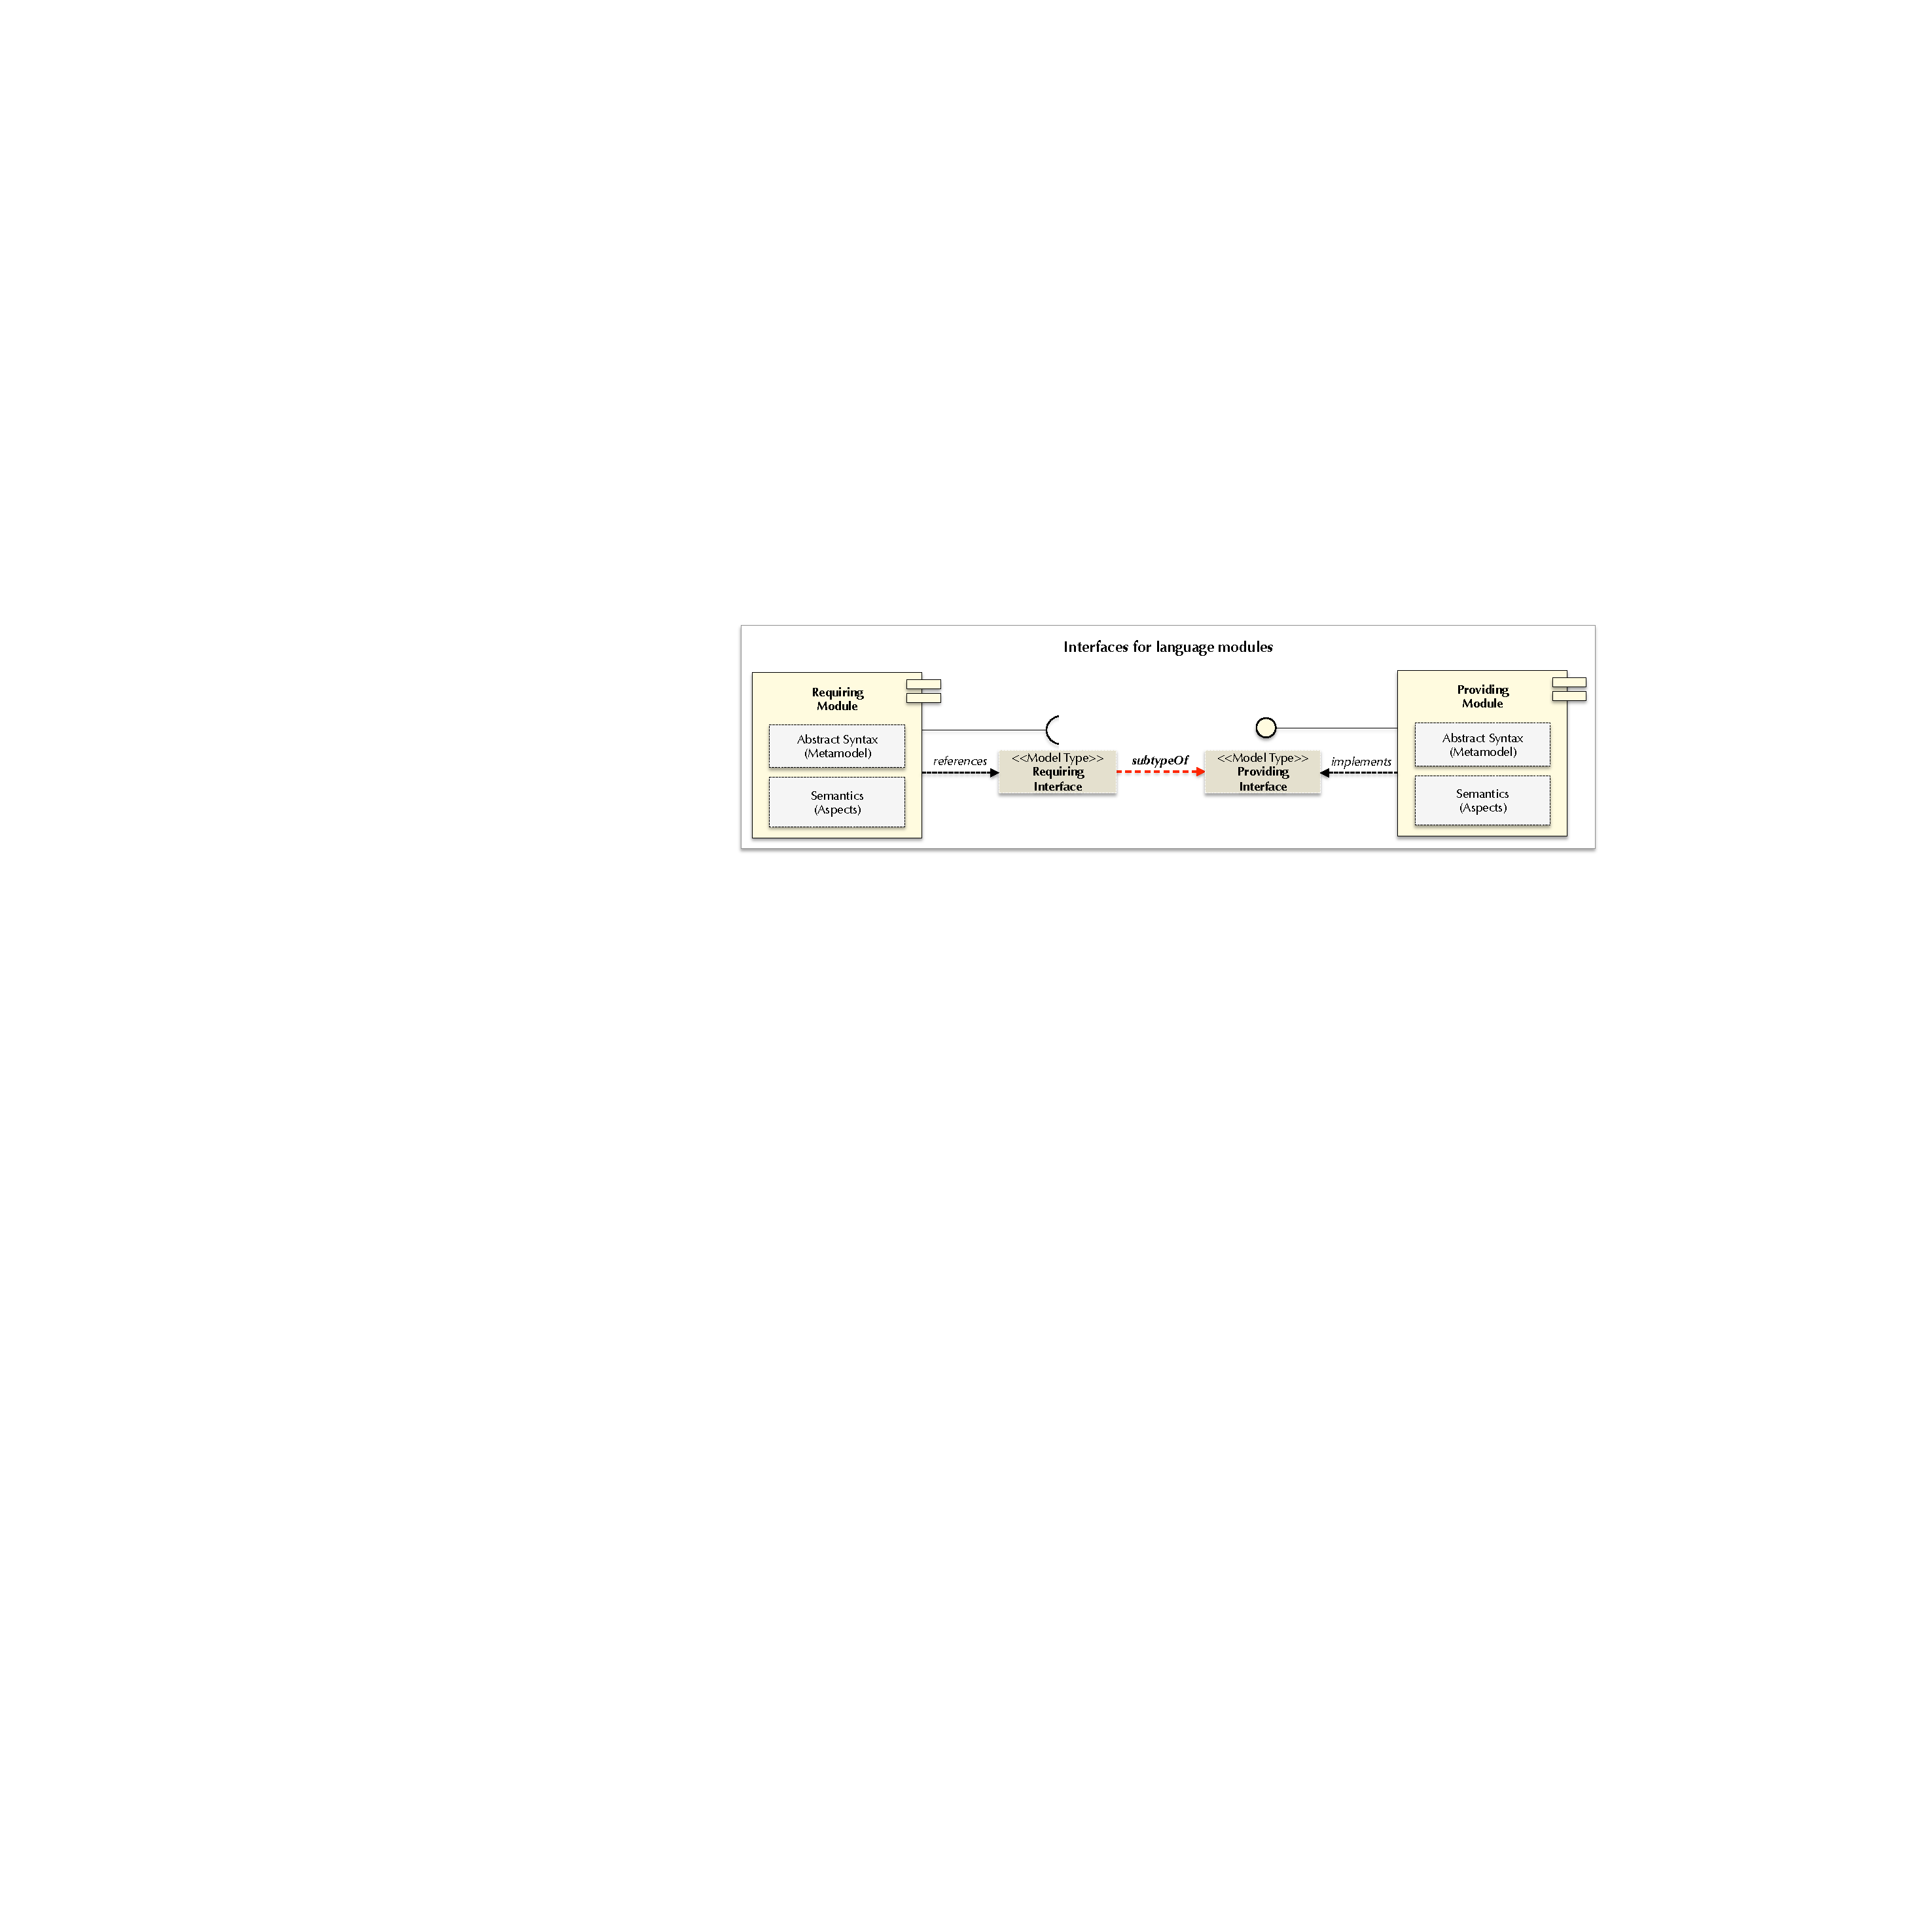
\includegraphics[width=1\linewidth]{images/approach-interfaces.pdf}
\caption{Interfaces for language modules}
\label{fig:approaches-interfaces}
\end{figure}

\vspace{-3mm}
\todo[inline]{Usa el ejemplo para ejemplificar... no te preocupes por el espacio. Despues recortamos... mira si esa figura puede ser mas pequenya}
%The tool support we provide for specifying interfaces on language modules is based on annotations at the level of the abstract syntax (i.e., the metamodel). That means that the required constructs of a requiring module are declared as meta-classes in the metamodel as the same as the actual constructs of the module. However, the required constructs are annotated with \texttt{@Required} to distinguish them from the actual constructs.